\section{STUFF - TODO}
\textcolor{red}{TODO}

\colorlet{mivertexcolor}{blue}
\colorlet{jivertexcolor}{red}
\colorlet{vertexcolor}{mivertexcolor!50}
\colorlet{bordercolor}{black!80}
\colorlet{linecolor}{gray}
% parameter corresponds to the used valuation function and can be addressed by #1
\tikzset{vertexbase/.style 2 args={semithick, shape=circle, inner sep=2pt, outer sep=0pt, draw=bordercolor},%
    vertex/.style 2 args={vertexbase={#1}{}, fill=vertexcolor!45},%
    mivertex/.style 2 args={vertexbase={#1}{}, fill=mivertexcolor!45},%
    jivertex/.style 2 args={vertexbase={#1}{}, fill=jivertexcolor!45},%
    divertex/.style 2 args={vertexbase={#1}{}, top color=mivertexcolor!45, bottom color=jivertexcolor!45},%
    conn/.style={-, thick, color=linecolor}%
}
\begin{figure}[H]
    \centering
    \begin{adjustbox}{max width=\textwidth}
        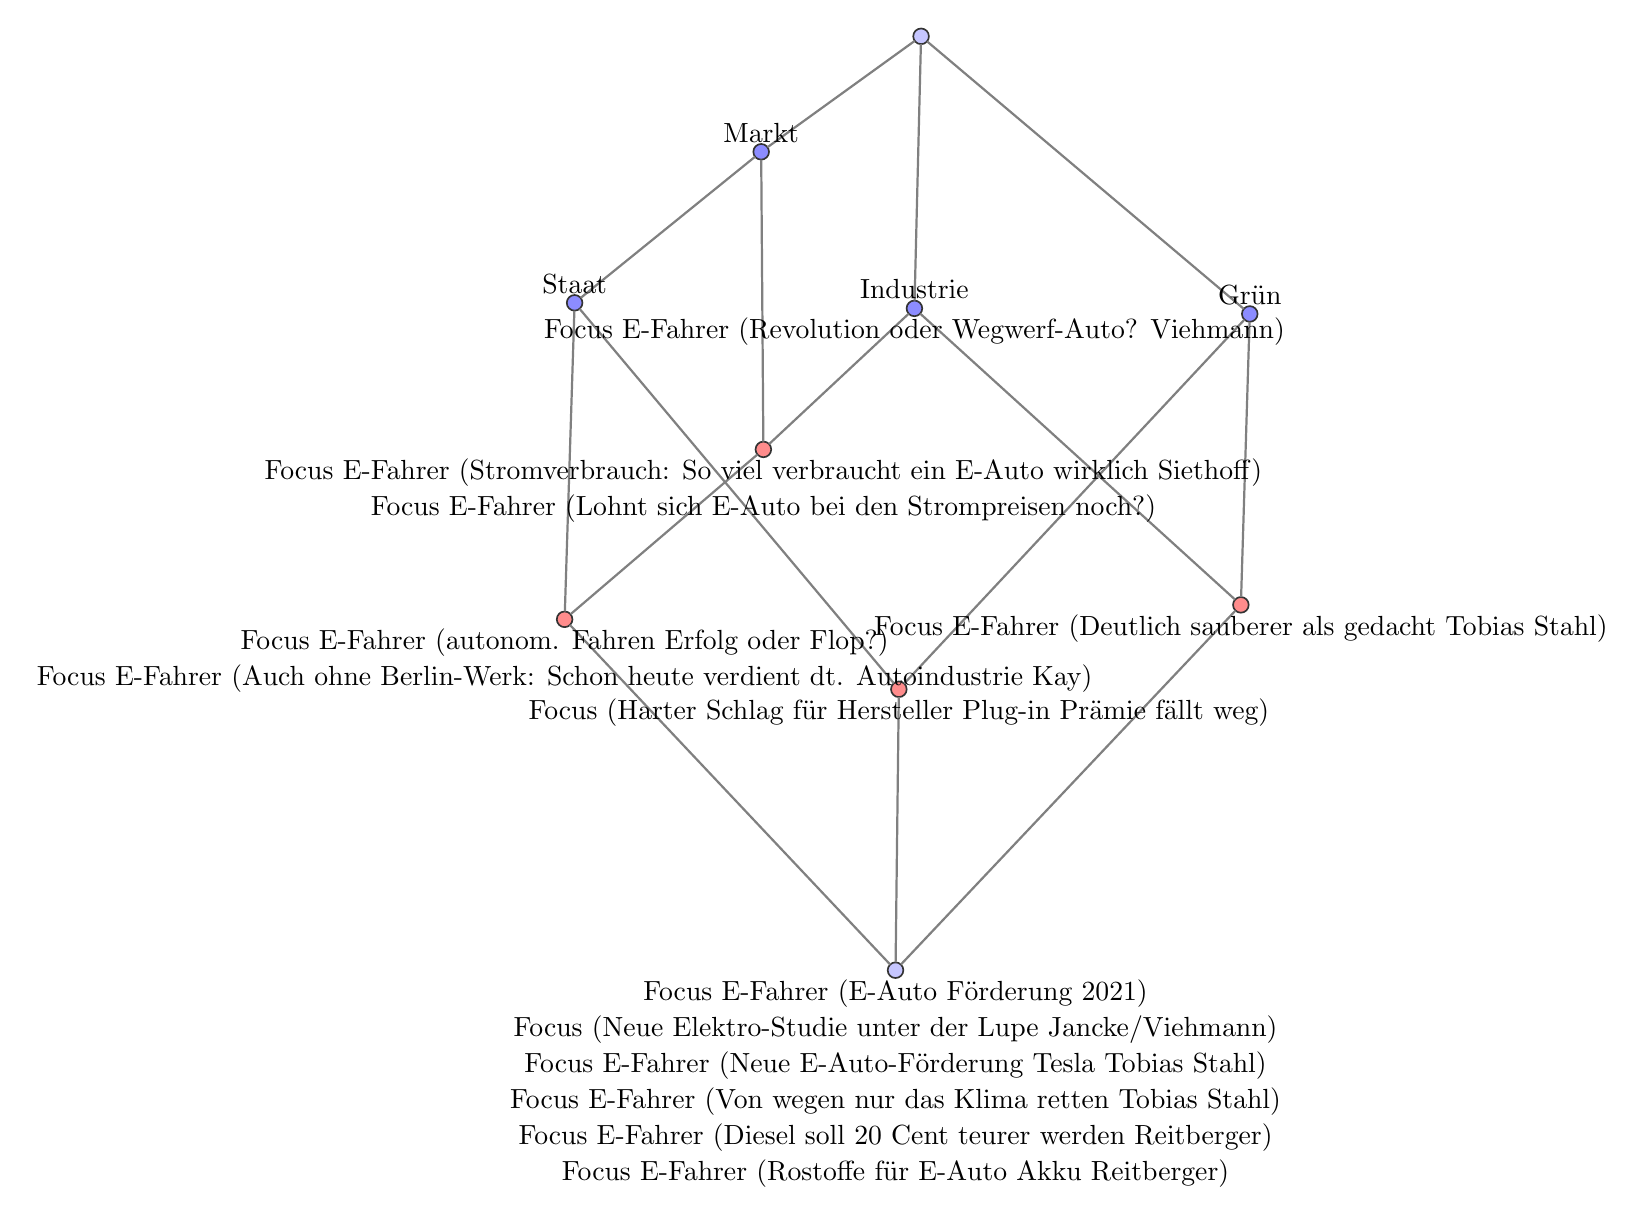
\begin{tikzpicture}
            \begin{scope} %for scaling and the like
                \begin{scope} %draw vertices
                    \foreach \nodename/\nodetype/\param/\xpos/\ypos in {%
                            0/vertex//-0.9525641025641018/2.73846153846155,
                            1/jivertex//-0.9102564102564106/6.306410256410267,
                            2/jivertex//-5.155128205128204/7.194871794871805,
                            3/jivertex//3.4333333333333336/7.378205128205138,
                            4/jivertex//-2.6307692307692303/9.352564102564113,
                            5/mivertex//3.546153846153846/11.073076923076933,
                            6/mivertex//-0.7128205128205121/11.143589743589754,
                            7/mivertex//-5.028205128205128/11.214102564102575,
                            8/mivertex//-2.6589743589743584/13.132051282051293,
                            9/vertex//-0.6282051282051277/14.598717948717958
                        } \node[\nodetype={\param}{}] (\nodename) at (\xpos, \ypos) {};
                \end{scope}
                \begin{scope} %draw connections
                    \path (8) edge[conn] (9);
                    \path (3) edge[conn] (5);
                    \path (3) edge[conn] (6);
                    \path (5) edge[conn] (9);
                    \path (0) edge[conn] (3);
                    \path (0) edge[conn] (1);
                    \path (0) edge[conn] (2);
                    \path (1) edge[conn] (5);
                    \path (1) edge[conn] (7);
                    \path (2) edge[conn] (4);
                    \path (2) edge[conn] (7);
                    \path (4) edge[conn] (8);
                    \path (4) edge[conn] (6);
                    \path (7) edge[conn] (8);
                    \path (6) edge[conn] (9);
                \end{scope}
                \begin{scope} %add labels
                    \foreach \nodename/\labelpos/\labelopts/\labelcontent in {%
                    5/above//{Grün},
                    6/above//{Industrie},
                    7/above//{Staat},
                    8/above//{Markt},
                    0/below//{\shortstack{Focus E-Fahrer (E-Auto Förderung 2021) \\ Focus (Neue Elektro-Studie unter der Lupe Jancke/Viehmann) \\ Focus E-Fahrer (Neue E-Auto-Förderung Tesla Tobias Stahl) \\ Focus E-Fahrer (Von wegen nur das Klima retten Tobias Stahl) \\ Focus E-Fahrer (Diesel soll 20 Cent teurer werden Reitberger) \\ Focus E-Fahrer (Rostoffe für E-Auto Akku Reitberger)}},
                    1/below//{Focus (Harter Schlag für Hersteller Plug-in Prämie fällt weg)},
                    2/below//{\shortstack{Focus E-Fahrer (autonom. Fahren Erfolg oder Flop?) \\ Focus E-Fahrer (Auch ohne Berlin-Werk: Schon heute verdient dt. Autoindustrie Kay)}},
                    3/below//{Focus E-Fahrer (Deutlich sauberer als gedacht Tobias Stahl)},
                    4/below//{\shortstack{Focus E-Fahrer (Stromverbrauch: So viel verbraucht ein E-Auto wirklich Siethoff) \\ Focus E-Fahrer (Lohnt sich E-Auto bei den Strompreisen noch?)}},
                    6/below//{Focus E-Fahrer (Revolution oder Wegwerf-Auto? Viehmann)}
                    } \coordinate[label={[\labelopts]\labelpos:{\labelcontent}}](c) at (\nodename);
                \end{scope}
            \end{scope}
        \end{tikzpicture}
    \end{adjustbox}
    \caption{\label{fig:fba-masterthesis}Begriffsverband - Masterarbeit}
\end{figure}

\begin{figure}[H]
    \centering
    \begin{adjustbox}{max width=\textwidth}
        \colorlet{mivertexcolor}{blue}
        \colorlet{jivertexcolor}{red}
        \colorlet{vertexcolor}{mivertexcolor!50}
        \colorlet{bordercolor}{black!80}
        \colorlet{linecolor}{gray}
        % parameter corresponds to the used valuation function and can be addressed by #1
        \tikzset{vertexbase/.style 2 args={semithick, shape=circle, inner sep=2pt, outer sep=0pt, draw=bordercolor},%
            vertex/.style 2 args={vertexbase={#1}{}, fill=vertexcolor!45},%
            mivertex/.style 2 args={vertexbase={#1}{}, fill=mivertexcolor!45},%
            jivertex/.style 2 args={vertexbase={#1}{}, fill=jivertexcolor!45},%
            divertex/.style 2 args={vertexbase={#1}{}, top color=mivertexcolor!45, bottom color=jivertexcolor!45},%
            conn/.style={-, thick, color=linecolor}%
        }
        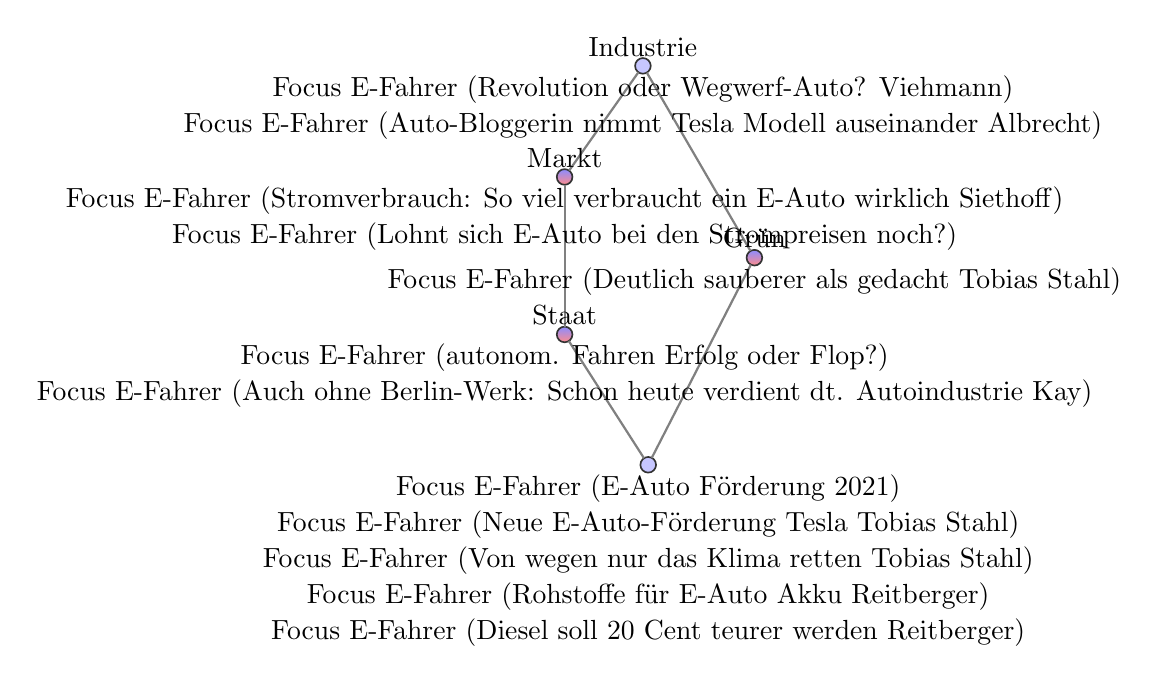
\begin{tikzpicture}
            \begin{scope} %for scaling and the like
                \begin{scope} %draw vertices
                    \foreach \nodename/\nodetype/\param/\xpos/\ypos in {%
                            0/vertex//0.061685823754787705/1.3448275862068968,
                            1/divertex//-1.0/3.0,
                            2/divertex//1.4103448275862052/3.9747126436781617,
                            3/divertex//-1.0/5.0,
                            4/vertex//-0.0057471264367841/6.4107279693486605
                        } \node[\nodetype={\param}{}] (\nodename) at (\xpos, \ypos) {};
                \end{scope}
                \begin{scope} %draw connections
                    \path (1) edge[conn] (3);
                    \path (3) edge[conn] (4);
                    \path (2) edge[conn] (4);
                    \path (0) edge[conn] (1);
                    \path (0) edge[conn] (2);
                \end{scope}
                \begin{scope} %add labels
                    \foreach \nodename/\labelpos/\labelopts/\labelcontent in {%
                    1/above//{Staat},
                    2/above//{Grün},
                    3/above//{Markt},
                    4/above//{Industrie},
                    0/below//{\shortstack{Focus E-Fahrer (E-Auto Förderung 2021) \\ Focus E-Fahrer (Neue E-Auto-Förderung Tesla Tobias Stahl) \\ Focus E-Fahrer (Von wegen nur das Klima retten Tobias Stahl) \\ Focus E-Fahrer (Rohstoffe für E-Auto Akku Reitberger) \\ Focus E-Fahrer (Diesel soll 20 Cent teurer werden Reitberger)}},
                    1/below//{\shortstack{Focus E-Fahrer (autonom. Fahren Erfolg oder Flop?) \\ Focus E-Fahrer (Auch ohne Berlin-Werk: Schon heute verdient dt. Autoindustrie Kay)}},
                    2/below//{Focus E-Fahrer (Deutlich sauberer als gedacht Tobias Stahl)},
                    3/below//{\shortstack{Focus E-Fahrer (Stromverbrauch: So viel verbraucht ein E-Auto wirklich Siethoff) \\ Focus E-Fahrer (Lohnt sich E-Auto bei den Strompreisen noch?)}},
                    4/below//{\shortstack{Focus E-Fahrer (Revolution oder Wegwerf-Auto? Viehmann) \\ Focus E-Fahrer (Auto-Bloggerin nimmt Tesla Modell auseinander Albrecht)}}
                    } \coordinate[label={[\labelopts]\labelpos:{\labelcontent}}](c) at (\nodename);
                \end{scope}
            \end{scope}
        \end{tikzpicture}
    \end{adjustbox}
    \caption{\label{fig:fba-smaller}Reduzierter Begriffsverband - Vorstudie}
\end{figure}